\documentclass{article}
\usepackage{tikz}
\usetikzlibrary{arrows.meta}

\begin{document}

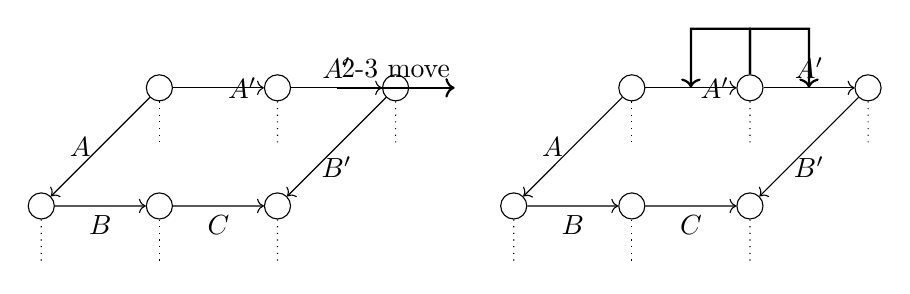
\begin{tikzpicture}[scale=1.5]
    % Nodes
    \node (A) at (0,0) [circle,draw] {};
    \node (B) at (-1,-1) [circle,draw] {};
    \node (C) at (0,-1) [circle,draw] {};
    \node (A') at (1,0) [circle,draw] {};
    \node (B') at (2,0) [circle,draw] {};
    \node (C') at (1,-1) [circle,draw] {};

    % Edges
    \draw[->] (A) -- node[left] {$A$} (B);
    \draw[->] (A) -- node[right] {$A'$} (A');
    \draw[->] (B) -- node[below] {$B$} (C);
    \draw[->] (A') -- node[above] {$A'$} (B');
    \draw[->] (B') -- node[below] {$B'$} (C');
    \draw[->] (C) -- node[below] {$C$} (C');

    % Dotted lines
    \draw[dotted] (A) -- ++(0,-0.5);
    \draw[dotted] (A') -- ++(0,-0.5);
    \draw[dotted] (B) -- ++(0,-0.5);
    \draw[dotted] (C) -- ++(0,-0.5);
    \draw[dotted] (B') -- ++(0,-0.5);
    \draw[dotted] (C') -- ++(0,-0.5);

    % Arrow for 2-3 move
    \draw[->,thick] (1.5,0) -- node[above] {2-3 move} (2.5,0);

    % Second part of the diagram
    \begin{scope}[xshift=4cm]
        % Nodes
        \node (A) at (0,0) [circle,draw] {};
        \node (B) at (-1,-1) [circle,draw] {};
        \node (C) at (0,-1) [circle,draw] {};
        \node (A') at (1,0) [circle,draw] {};
        \node (B') at (2,0) [circle,draw] {};
        \node (C') at (1,-1) [circle,draw] {};

        % Edges
        \draw[->] (A) -- node[left] {$A$} (B);
        \draw[->] (A) -- node[right] {$A'$} (A');
        \draw[->] (B) -- node[below] {$B$} (C);
        \draw[->] (A') -- node[above] {$A'$} (B');
        \draw[->] (B') -- node[below] {$B'$} (C');
        \draw[->] (C) -- node[below] {$C$} (C');

        % Dotted lines
        \draw[dotted] (A) -- ++(0,-0.5);
        \draw[dotted] (A') -- ++(0,-0.5);
        \draw[dotted] (B) -- ++(0,-0.5);
        \draw[dotted] (C) -- ++(0,-0.5);
        \draw[dotted] (B') -- ++(0,-0.5);
        \draw[dotted] (C') -- ++(0,-0.5);

        % Arrows for 2-3 move
        \draw[->,thick] (A') -- ++(0,0.5) -- ++(-0.5,0) -- ++(0,-0.5);
        \draw[->,thick] (A') -- ++(0,0.5) -- ++(0.5,0) -- ++(0,-0.5);
    \end{scope}
\end{tikzpicture}

\end{document}